\documentclass{UoNMCHA}

% Packages to include
\usepackage[authoryear]{natbib}
\usepackage{array,booktabs} % For nice tables
\usepackage{amsmath,amsfonts,amssymb,mathrsfs,bm} % For nice 
\usepackage{color}
\usepackage{enumerate}
\usepackage{listings}
\usepackage{subfig}
\usepackage{hyperref}
\usepackage[normalem]{ulem}
\usepackage[parfill]{parskip}   % For replacing paragraph indenting with a newline instead

\usepackage{csvsimple} % For tables from CSV
\usepackage{float} % Used for forcing diagrams to the [H] action
% Wikipedia-style "citation needed" macro source: https://gist.github.com/martinarroyo/b9e0a963ad27169a6eee
\newcommand{\citationneeded}{\textsuperscript{\color{blue} [citation needed]}}
% \renewcommand{\floatpagefraction}
%from/for unicode-math
%\setmathfont{texgyrepagella-math.otf}[math-style=TeX]

% New macro to make defining labels easier.
%\newcommand{\citationneeded}{\textsuperscript{\color{blue} [citation needed]}}
\newcommand{\inlineQuote}[1]{``#1''}


\newcommand{\fref}[1] {Figure: \ref{#1}}

\newcommand{\fFigure}[3]{
	\begin{figure}[h]
        \begin{center}  
            \includegraphics[width=#3\linewidth]{Figures/#1}  
            \caption{#2}
            \label{#1}
        \end{center}
	\end{figure}
}

% \fref{TEST.png}
% \fFigure{TEST.png}{caption}{0.8}

% \newcommand{\cFigure}[4]{
%     \begin{figure}[h]
%         \begin{center}
%             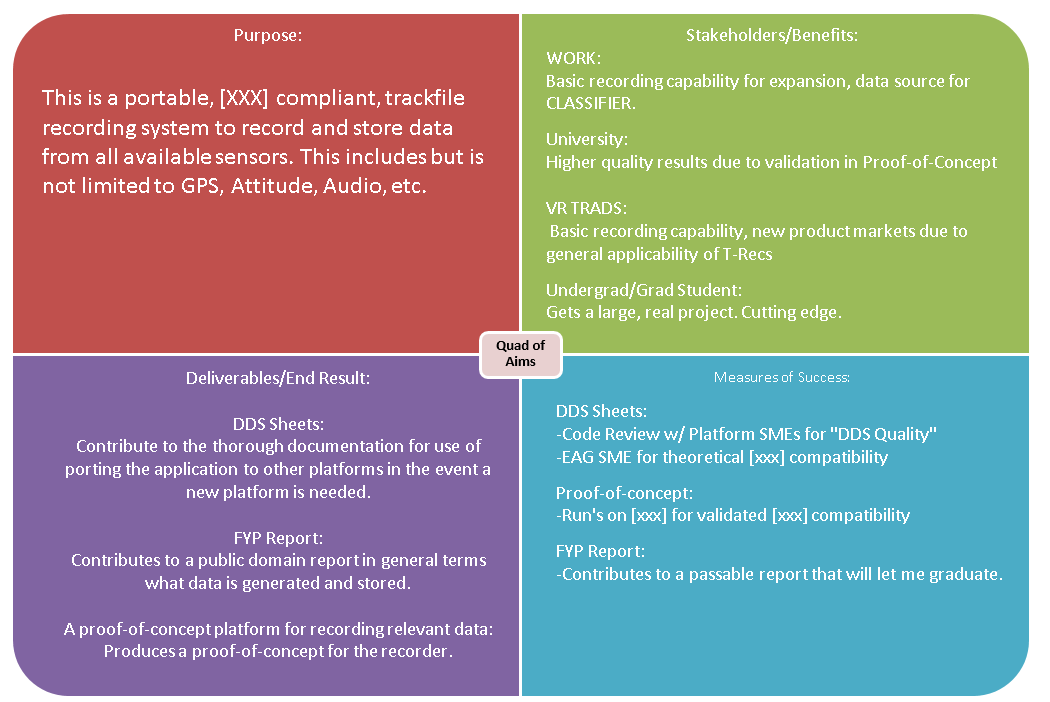
\includegraphics[width=0.8\linewidth]{Figures/QuadOfAims2.png}
%             \caption{A Quad of Aims for the project might be A3 in size and would have the relevant information embedded. It may also be completed on a white-board.}
%             \label{fig:AndroidDataExample}
%         \end{center}
%      \end{figure}    

% \begin{figure}[h!]
% 		\label{\getLabel{#2}{#3}{#4}}
% 		 \centering
% 		 \includegraphics[width=\linewidth]{#1}	 
% 		 \caption{#2 for #4 DOF mesh, Re #3.}
% 	\end{figure} 
% }



 

%\LoadClass[twoside,a4paper,11pt]{scrartcl}

% Make all math bigger
%\setmathfont{XITS Math}[10pt,version=xits]

%\defaultscriptratio=0.7

% Number equations per section
\numberwithin{equation}{section}

\hypersetup{
%    bookmarks=true,         % show bookmarks bar?
%    unicode=false,          % non-Latin characters in AcrobatÕs bookmarks
%    pdftoolbar=true,        % show AcrobatÕs toolbar?
%    pdfmenubar=true,        % show AcrobatÕs menu?
%    pdffitwindow=false,     % window fit to page when opened
%    pdfstartview={FitH},    % fits the width of the page to the window
    pdftitle={FYP Report - Trackfile Recording System},    % title
    pdfauthor={Chris Caelli},     % author
    pdfsubject={FYP PART B},   % subject of the document
%    pdfcreator={Creator},   % creator of the document
%    pdfproducer={Producer}, % producer of the document
%    pdfkeywords={keyword1} {key2} {key3}, % list of keywords
%    pdfnewwindow=true,      % links in new window
    colorlinks=true,       % false: boxed links; true: colored links
    linkcolor=blue,          % color of internal links
    citecolor=blue,        % color of links to bibliography
%    filecolor=magenta,      % color of file links
    urlcolor=blue           % color of external links
}

\definecolor{MATLABKeyword}{rgb}{0,0,1}
\definecolor{MATLABComment}{rgb}{0.1328125,0.54296875,0.1328125}
\definecolor{MATLABString}{rgb}{0.625,0.125,0.9375}

\lstset{language=Matlab,
    basicstyle=\small\ttfamily,
    keywordstyle=\color{MATLABKeyword},
    %identifierstyle=,
    commentstyle=\color{MATLABComment},
    stringstyle=\color{MATLABString},
    numberstyle=\tiny,
    %numbers=left,
    basewidth=0.5em}




\firstpage{1}    % Set page number for first page
\UoNMCHAreportNo{MECH4841 Part B} %Report number
\UoNMCHAyear{2019}   % Year
\shorttitle{FYP Report - TRecS} %For odd pages
%%%%%%%%%%%%%%%%%%%%%%%%%%%%%%%%%%%%%%%%%%%%%%%%%%%%
\begin{document}
\title{FYP Report - Trackfile Recording System \\ \ \\
{\small Final Year Project Report - MECH4841 Part B  \\MAY 2019}}
\author[UoNMCHA]{Christopher Caelli}
\address[UoNMCHA]{
Student of Mechatronics Engineering,\\
The University of Newcastle, Callaghan, NSW 2308, AUSTRALIA \\
Student Number: 3206246 \\
E-mail: \href{mailto:Christopher.Caelli@uon.edu.au}{\textsf{Christopher.Caelli@uon.edu.au}}}
%%%%%%%%%%%%%%%%%%%%%%%%%%%%%%%%%%%
\maketitle
\onecolumn

\vspace{-5mm}
\section*{Mandatory Dot Point Summary}
\vspace{-3mm}
As per the FYP Handbook: \newline
I did:
\begin{itemize}
    \item I learnt and prototyped a machine learning algorithm for classifying physical actions from an audio input
    \item I investigated prototyping a machine learning solution that takes audio and physical data (GPS, accelerometer, gyroscope) to compare whether subject matter insight could improve the classification of sound. That is, would a mechatronics understanding help in pre-processing or improving the data source, resulting in better classification?
    \item I used my mechatronics subject matter learnings to best apply machine learning to this problem. This includes Mechatronics Design (trade off and evaluations from MCHA3000), sound pre-processing, preprocessing Inertial Measuring Unit data, and how Audio waveforms can be treated as energy.
    \item I learnt and used System Engineering techniques to elicit requirements from my university and work stakeholders
\end{itemize}
I helped:
\begin{itemize}
   \item I managed and worked with another employee to implement a proof of concept app to record data as an input into a this project. This involved using my software engineering skills and project management skills to create a schema, develop the android app, and present it to the relevant stakeholders.
%    \item 
%     \item \sout{I helped integrate this proof of concept with a larger C\# replay system at my work. This involved lat/long coordinate calculations for display playback, leading the configuration management with a local git server, and helping develop the data pipeline where the proof of concept feeds through my machine learning classifier, and into the larger replay system.}
\end{itemize}
\newpage

%%%%%%%%%%%%%%%%%%%%%%%%%%%%%%%%%%%
\vspace{-5mm}
\section*{Executive summary}
\vspace{-3mm}
The project investigated whether using data from an Inertial Measurement Unit (IMU) and GPS data as additional data points in an Acoustic Event Detection / Classification (AED/C) problem would improve a classifier's ability to classify an “acoustic event”. The motivation behind this was to improve AED/C without onerous microphone requirements. The project began documenting the process of evaluating the research problem for a car use case (specific tasks such as putting on a seatbelt, closing doors, indicating, horn use, etc.). This includes the requirements, data collection, data pre-processing, design and training of the classifier, and evaluating the results. Due to a lack of data, the public ExtraSensory dataset was used for the AED/C for similar events such as walking, driving, sleeping, computer work, etc. to demonstrate the researched technologies. Results show the supplementary data improved classification. This research shows multi-sensor AED/C is effective but requires more datasets.
% This document will cover the author's progress through the Final Year Project. The scope of the project is a portable data recording system coupled with offline processing to track and identify specific physical events in close proximity that occurred during recording. Acoustic Event Detection and Classification is the focus of this paper, and the goal of this FYP report is exploring and validating current research techniques in an uncontrolled environment for a specific use case. The content of this paper will start with, system engineering, problem analysis, a review into the current research and will expand to document python implementation, machine learning, data pre-processing, app development and progress in developing the proof of concept to take logged data from a phone and process it on a sever to create a “trackfile” (special csv file).

%%%%%%%%%%%%%%
\vspace{-2mm}
\section*{Acknowledgements}
\vspace{-3mm}
I'd like to thank my partner Brigid for encouraging and supporting me throughout this project.
\newpage
\tableofcontents
\newpage
%%%%%%%%%%%%%%%%%%%%%%%%%%%%%%%
\section{Introduction}
Debriefing is a tool used to educate an individual, inform a collective and create a holistic historical recording of an event. Wikipedia defines the process of debriefing as: (1) Receiving an explanation, (2) Receiving information and situation-based reminders of context, (3) Reporting of measures of performance, and/or opportunities to further investigate the results of a study, investigation, or assessment of performance after participation in an immersive activity is complete\citationneeded. Traditionally this is done through a collection of primary sources (where available) and secondary sources. In the information age, these primary sources have expanded to include large datasets, recordings and other digital forensics. This new and increasing range of primary sources provides the potential to significantly improve the steps of debriefing, and ultimately improve debriefing outcomes.

This paper will report on the Author’s progress of harnessing this new potential and is organised as follows: section 2 will discuss how the scope has been analysed and reduced, section 3 will review the literature of this research topic, section 4 will discuss the method of implementing the technology, section 5 will discuss the evaluation methodology, and section 6 will discuss the results of the proof-of-concept.

% To organise your introduction section you can use the following structure:
% \begin{itemize}
%     \item \textbf{Position}: Show there is a problem and that it is important to solve it.
%     \item \textbf{Problem}: Describe the specifics of the problem you are trying to address
%     \item \textbf{Proposal}: Discuss how you are going to address this problem. Use the literature to back-up your approach to the problem, or to highlight that what you are doing has not been done before
% \end{itemize}
% Here you need to sell why what you are doing is important, and what benefits will it bring if you are successful and solve the problem? 
%

%%%%%%%%%%%%%%%%%%%%%%%%%%%%%%%
\section{Problem Analysis}\label{sec:ProblemAnalysis}

This project approached the problem through a System Engineering perspective, a process which “is a structured and systematic methodology providing greater visibility and control over … new system[s]” \citationneeded [2]. This perspective was informed by ISO 15288 \citationneeded [3] and Burge Hughes Walsh’s System Engineering Toolbox \citationneeded [4]. The tools adapted and applied throughout this section are primarily derived from that \inlineQuote{System Engineering Toolbox}. 

% \subsection{Purpose of Problem Analysis} %should this be a 
The purpose of Problem Analysis is to define the scope of this project to be achievable, measurable and practical to implement. This took 2-4 weeks through June 2018, and remains an ongoing task. 

% \subsection{System Engineering Tools for Problem Analysis}
The following System Engineering tools have been adapted and implemented to develop this paper and the author’s understanding of the problem. 

\subsection{Current 18 Words}
A tool called \inlineQuote{18 Words} was used to constantly refine and maintain a description on the scope as it changed throughout problem analysis. The current “18 Words” is the following:
“[The project is] a portable proprietary format compliant track file data recording system coupled with offline processing to log specific physical events in proximity that occurred during recording.” 

\subsection{Tree Diagram}
With the new understanding of what the project is, a Tree Diagram was drafted to explore missed requirements, hidden modules and other aspects of the project not yet considered. \fref{treeDiagram.png} shows a Tree Diagram breakdown for this FYP.

 \fFigure{treeDiagram.png}{A tree diagram for the project, being used as a method of allocating work}{0.7}


\subsection{Quad of Aims}
The Quad of Aims is a tool used to explore 4 critical, high level aspects of the project as explained in table \ref{tab:QuadOfAims}, and shown in \fref{QuadOfAims2.png}.

\fFigure{QuadOfAims2.png}{A Quad of Aims for the project might be A3 in size and would have the relevant information embedded. It may also be completed on a white-board.}{0.7}

 \begin{table}[h]
    \begin{center}
        \caption{Quad of Aims }\label{tab:QuadOfAims}
        {\footnotesize
            \begin{tabular}{c l l l|}
                \hline\hline Label & Description \\ \hline 
                Purpose & This is our “18 words” \\
                Stakeholders & University, Author’s Work \\
                Deliverables & Documentation, recommendations, FYP report, proof-of-concept \\
                Measure of Success & Review of Documentation by SMEs, review of FYP report, dry and wet run of proof-of-concept \\
                \\ \hline
            \end{tabular}
        }
    \end{center}
\end{table}

This is typically done to instigate early works on a project.

\subsection{Input Output Analysis}
The Input Output Analysis of the system informs the bounds and requirements to operate the system. In this situation, it helped consider the full scope of the project; this includes the technical and non-technical aspects of undertaking the MECH4841 Project as shown in \fref{InputOutput.png}.

\fFigure{InputOutput.png}{The input output analysis for the system}{0.75}


\subsection{Affinity Diagram}
An Affinity Diagram helps to solidify the high level, vague ideas, requirements and tests into a more detailed view. There is a focus on putting tangible measurements onto requirements. During this process, system architecture decisions were made such as a trade review into online vs offline processing, and subsequently splitting the system into smaller modules. Our primary system had 2 key sub-systems: The recording, and the processing systems. An Affinity Diagram of the top-level sys-tem was created, and the 2 affinity diagrams of the sub-systems were informed and made from this. After this was complete, previous work was updated to reflect these changes. *ADD A REF TO THE FIGURE* \fref{AffinityDiagram.png}
\fFigure{AffinityDiagram.png}{The Affinity Diagrams for the full system architecture}{0.8}

\subsection{Systems Map}
A Systems Map takes the Affinity Diagram, Input Output Analysis, and Tree-Diagram to identify the processes inside sub-modules that are needed to design the system. This was used to great effect to measure and estimate the workload necessary to implement data fusion alongside deep learning of acoustic classification and detection as shown in \fref{SystemMap.png}.
\fFigure{SystemMap.png}{A systems map for the project}{0.8}


\subsection{Sequence Diagram}
A Sequence Diagram was developed to analyse the flow of data through the processes identified in the System Map. This is shown in \fref{SequenceDiagram.png}. This helped to predict and manage any potential complexities and logistics related to the specific needs of each process. 
Originally, This Sequence Diagram was used to justify removing data fusion from the scope due to the large workload required to implement alongside machine learning. Later in the project, it was brought back into the scope of the project to help compare and evaluate it's effectiveness in improving the overall system. 
\fFigure{SequenceDiagram.png}{A basic Sequence Diagram for the project}{0.8}


\subsection{N\textsuperscript{2} Analysis}
An N\textsuperscript{2} Analysis methodically expands on the what data moves around the system. This is to compliment the discussed complexities in the Sequence Diagram by documenting what data is expected. A example of this is shown in \fref{n2analysis.png}
\fFigure{n2analysis.png}{A N\textsuperscript{2} Analysis for the project}{0.8}

\subsection{Spray Diagram}
The Spray Diagram shown in \fref{SprayDiagram.png} shows how details of the system can have multi-factored effects in design requirements, outcomes and operational use. Of interest in the diagram is the relationship between high-quality output will require high-quality input, and this may increase production and design costs. 
\fFigure{SprayDiagram.png}{A Spray Diagram for the project}{0.8}

\subsection{Matrix Diagram}
A matrix diagram was made to review the now more refined, reduced scope as shown in \fref{MatrixDiagram.png}. This works by using a “strong”, “weak” or “none” indicator for each aspect of the project. It highlighted the difficulty in balancing the needs of both major stakeholders. 
\fFigure{MatrixDiagram.png}{A Matrix Diagram for the project}{0.8}

\subsection{Final Problem Analysis}
\subsection{Discussion}
The purpose of the project is to hypothesis and produce a proof-of-concept of how digital technologies could improve debriefing processes and outcomes. This seems achievable within 1 year, and should provide an excellent learning opportunity for the author.

%%%%%%%%%%%%%%%%%%%%%%%
\section{Review Of Literature}
A literature review of the current research was conducted with guidance from University of Queensland’s guide to Literature reviews [5] \citationneeded . There are 3 nested areas of research that are of interest to this project. The wider classification and regression research topic, the machine learning topic that covers many various fields of implemented and theoretical machine learning applications, and finally the specific field of Acoustic Event Detection and Classification (AED/AEC); this field has traditionally relied on older techniques, and is undergoing a revolution with machine learning. 
\fFigure{niche.png}{The literature for this project is a niche topic in the Machine Learning area of research}{0.8}

\subsection{Machine Learning}
A definition for Machine learning is taken from Tom M. Mitchell's 1997 textbook, \inlineQuote{Machine Learning}
\begin{quote}
    A computer program is said to learn from experience E with respect to some task T and some performance measure P, if its performance on T, as measured by P, improves with experience E. \citationneeded
\end{quote} /citationneeded  Mitchell, T. (1997). Machine Learning. McGraw Hill. p. 2. ISBN 978-0-07-042807-2.

This definition of Machine Learning lends itself to best explaining this project; The task T (AED/C), the E (Audo, IMU, GPS), and P (a traditional F1 score). 

The computer program described in this project has been produced in Python, using the sklearn and tensorflow libraries.

\subsection{Acoustic Event Detection and Acoustic Event Classification}
Historically the technologies for AED/AEC have been Support vector machine (SVMs), Hidden Markov Models (HHMs), and more generally, basic DSP (Digital Signal Processing) classifiers. But in the last 8 years, AED and AEC research has emerged as a hot topic of research. Research focuses on the two key tasks: Detection (when did an acoustic event occur in the au-dio, and when did it stop?) and classification (what sound oc-curred?). New research papers are often the result of DCASE competitions, which is an official IEEE Audio and Acoustic Signal Processing (AASP) competition.
\fref{F1_score.png}
\fFigure{F1_score.png}{DCASE Researcher Toni Heittola's F1 Results reflect the AED/AEC field of research with drastic improvements over the last 8 years. \citationneeded}{0.8}

\subsection{DCASE Competitions (Detection and Classification of Acoustic Scenes and Events)}
The DCASE competitions format started 2013, had its second competition in 2016, and since then has been a yearly event. Since 2017, there has been a new format where the competi-tion starts march, formal results are released by September, and a workshop for participants on the best team’s work in Novem-ber [7]. 2016 was the first to feature Machine Learning (win-ning teams incorporated machine learning into ensemble mod-els/classifiers). By 2017 all entries utilised machine learning. Recently the results from DCASE2018 have been published; progress in the AED/AEC field has allowed more sophisticated, real-world applications to be evaluated (Challenge Task \#4) [8]. The complexity of the dataset, the number of acoustic classes and fidelity of output are unprecedented in the AEC field. The winning results at this level of complexity aren’t as high quali-ty compared to last year’s more controlled environment/dataset (2017 had a 41.7\% F1 score [9] vs 2018’s 32.4\% [8]), but pre-sent the best precedent for the problem addressed in this paper.

\subsection{Leading Research, DCASE2018 Task 4 Winner}
The winning model used in the DCASE2018 Task 4 challenge used a “Mean-teacher” model for classification (useful abstract results averaging applicable to a range of classifier models), a CNN for context gating (a pre-classifier step to improve flaws in training methodologies for some machine learning models [10]) and a bidirectional recurrent neural network (RNN) to improve the utilisation of unlabelled, unbalanced training da-tasets [11]; this last component is important for this paper, as the leading dataset outside of DCASE challenges is the weakly labelled Google AudioSet, of which only small percentage of is balanced.

\begin{table}[h!]
    \begin{center}
        \caption{AudioSet data on Cars}\label{tab:AudioSetCars}
        {\footnotesize
            \begin{tabular}{c l l l|}
                \hline\hline Dataset & Number of videos & Duration hours \\ \hline 
                Evaluation & 280 & 0.8 \\
                Balanced train & 296 & 0.8 \\
                Unbalanced train & 40,978 & 113.3 \\
                Overall & 41,554 & 114.9 \\
                \\ \hline
            \end{tabular}
        }
    \end{center}
\end{table}
\begin{gather*}
    Car AudioSet:  \frac{0.8}{114.9}=0.69\%
\end{gather*}

%%%%%%%%%%%%%%%%%%%%%%%
\section{Method}
The method for learning and prototyping the Machine Learning interface was driven by reading [some textbook], and then building up the network in small stages. The desired topology was the Mean Teacher topology from DCASE 2018, however it was beneficial to work up slowly to this goal.  The main tasks required to build the classifier are as follows:

\begin{itemize}
    \item Develop the use-case, and identify the output
    \item Investigate what datasets are available, and whether further data would be beneficial
    \item Choose a framework/technology to implement the machine learning algorithm in
    \item Build the machine learning, and test it's effectiveness
    \item Refine the network using the F-Score
    \item Take the classified output, and append it to the input trackfile
\end{itemize}

\subsection{Required Data}
The Machine Learning uses GPS, accelerometer, gyroscope, and audio. A Google Pixel 2 was selected as the model data acquisition, which table /ref{} below shows.
\begin{table}[h!]
    \begin{center}
        \caption{Data Available\citationneeded}\label{tab:AndroidDataAvailable}
        {\footnotesize
            \begin{tabular}{c l l l|}
                \hline\hline Sensor & Description \\ \hline 
                GPS & The Pixel 2 uses the Snapdragon 835 System on Chip GPS receiver\\
                Accelerometer / Gyroscope & The Pixel 2 uses a bosch BMI160 \\
                Audio & The Pixel 2 uses a Qualcom WCD9395 Audio Codec chip, a NXP TFA9891UK Audio Amplifier, \citationneeded FINISH \\
                \\ \hline
            \end{tabular}
        }
    \end{center}
\end{table}

\subsection{Data Collection}

The choice of what data to collected and use was found through the first problem analysis step. As the goal is to maximise the accuracy of the classifier (whilst still being an achievable goal), the data chosen for use and collection was GPS, accelerometer, gyroscope, and audio. As described in the problem analysis phase, the best platform for this would be a smartphone as shown in section \ref{sec:ProblemAnalysis} and appendix \ref{sec:TradeReview}. 

% The choice of what data to collected and use was found through the first problem analysis step. As the goal is to maximise the accuracy of the classifier (whilst still being an achievable goal), the data chosen for use and collection was GPS, accelerometer, gyroscope, and audio. As described in the problem analysis phase, the best platform for this would be a smartphone as shown in section \ref{sec:ProblemAnalysis} and appendix \ref{sec:TradeReview}. 

Android was chosen as the platform as it had significant support for reading from the on-board sensors. The data available from the Android API can be seen in table \ref{tab:AndroidDataAvailable}, of which GPS and acceleration will be used. It was also chosen due to it's support for C/C++ through the Native Development Kit (NDK). The programming language C is required knowledge for many courses in the University of Newcastle Bachelor of Mechatronics degree. 

The app development took 5 weeks to get to a useful state. It is able to record Audio to a .wav file and record raw GPS lat/long/alt, raw accelerometer, and raw gyroscope to a csv. There are technical issues still present in the app (notably that the screen must be unlocked to record).

During this time, an Atlassian JIRA environment was set up to facilitate management (using concepts from ENG3500 - Project Management). The Atlassian "Git-Flow" methodology was also learnt and used.

I helped with 30\% of the overall programming, and code reviewed the product along with other colleagues. Credit goes to [Sebastian Wallman].

\subsubsection{Data collected during project vs ExtraSensory datset}
The table \ref{tab:ProjectData} shows a snippet of the Comma-Seperated Values (csv) data produced from the app. The id is a unique count, %the attr\_time is a timestamp from the Android system, and attr\_x, attr\_y, and attr\_z are the raw output of the. 
The table \ref{tab:ExtraSensoryData} shows a snippet of the csv data from the ExtraSensory dataset. 

Both datasets share the same timestamp format, so a \inlineQuote{Time} column has been added to the table for illustration purposes only.

%https://developer.android.com/guide/topics/sensors/sensors_motion
 \lstinputlisting[
    language=C,
    float=h,
    numbers=left,
    xleftmargin=1cm,
    frame=shadowbox,
    caption={Code snippet for getting Accelerometer data from the Android System as above \citationneeded above},
    morekeywords={try,catch}
    ]{accel_example.c}


\begin{table}[]\label{tab:ProjectData}
    \begin{center}
        \begin{tabular}{llllll}
        \hline\hline id & attr\_time & Time & attr\_x   & attr\_y & attr\_z \\ \hline
        1  & 1547182324433 & 2018-01-11 14:52 & -0.229843 & 3.1795  & 8.52336 \\
        2  & 1547182324442 & 2018-01-11 14:52 & -0.257614 & 2.93185 & 8.61444 \\
        3  & 1547182324451 & 2018-01-11 14:52 & -0.179626 & 2.81464 & 8.81348 \\
        4  & 1547182324467 & 2018-01-11 14:52 & -0.118927 & 2.82674 & 8.70142 \\
        5  & 1547182324498 & 2018-01-11 14:52 & -0.191544 & 2.95287 & 8.66815 \\ \hline
        \end{tabular}
    \end{center}
\end{table}


\begin{table}[]\label{tab:ExtraSensoryData}
    \begin{center}
        \begin{tabular}{lllllll}
            \hline\hline timestamp  & Time & raw\_acc:mean & raw\_acc:std & raw\_acc:moment3 & raw\_acc:moment4 \\\hline 
        1464129912 & 2016-05-24 22:45 & 1.011438                       & 0.012573                      & 0.023013                          & 0.04124      \\
        1464129950 & 2016-05-24 22:45 & 1.011233                       & 0.009356                      & -0.005622                         & 0.016687     \\
        1464130031 & 2016-05-24 22:47 & 1.013422                       & 0.018068                      & -0.008593                         & 0.039286     \\
        1464130109 & 2016-05-24 22:48 & 1.014891                       & 0.0164                        & 0.021383                          & 0.038825     \\
        1464130130 & 2016-05-24 22:48 & 1.017487                       & 0.022632                      & -0.012891                         & 0.037226    \\\hline 
        \end{tabular}
    \end{center}
\end{table}

The ExtraSensory dataset is compiled from 60 users with a diverse range of phones (\inlineQuote{34 iPhone users, 26 Android users.}\citationneeded http:\/\/extrasensory.ucsd.edu\/). This is in contrast to this project's phone range, which was limited to 2 Android devices, a Samsung S6 and a Lenovo Zuk Z2. The Samsung uses a InvenSense MPU-6500, the Lenovo Zuk Z2 unknown.

\begin{quotation}
    \underline{Devices:}
    The users in ExtraSensory had a variety of phone devices.
    iPhone generations: 4, 4S, 5, 5S, 5C, 6 and 6S.
    iPhone operating system versions ranging from iOS-7 to iOS-9.
    Android devices: Samsung, Nexus, HTC, moto G, LG, Motorola, One Plus One, Sony.
\end{quotation}


\subsection{Data Pre-Processing}
Python was used to process the data before the Machine Learning modules of code, and Matlab was used with GPS, IMU to prototype the algorithms. 


 \sout{The data from the ExtraSensory dataset is provided in it's raw format, which is best option is for the data to be raw, as this allows platform independent filtering, smoothing and sensor fusion\citationneeded.} 

\subsubsection{Audio}
Data preprocessing of the Audio was done by Mel Frequency Cepstral Coefficents (MFCC). Start with a recorded .wav sample, and split the whole sample into smaller sections via the sliding window method\citationneeded. Take each window and calculate the Fourier transform.
\begin{gather}%\label{eq:EquationLine}
    WindowSample(t) \xrightarrow{\mathscr{F}}  WindowSample(\omega)
\end{gather}

\lstinputlisting[
    language=Matlab,
    float=h,
    numbers=left,
    xleftmargin=1cm,
    frame=shadowbox,
    caption={Matlab trial of MFCC extraction\label{lst:matlabMFCC}},
    morekeywords={try,catch}
    ]{code/extract_mfcc.m}

% \textbf{!!!!from Wikipedia!!!}
% \begin{enumerate}
%     \item \sout{Take the Fourier transform of (a windowed excerpt of) a signal.}
%     \item \sout{Map the powers of the spectrum obtained above onto the mel scale,using triangular overlapping windows.}
%     \item \sout{Take the logs of the powers at each of the mel frequencies.}
%     \item \sout{Take the discrete cosine transform of the list of mel log powers, as if it were a signal.}
%     \item \sout{The MFCCs are the amplitudes of the resulting spectrum.}
% \end{enumerate}

Audio to a .wav file and record raw GPS lat/long/alt, raw accelerometer, and raw gyroscope to a csv.  

“First, resample the audio clips at 22,050 Hz, because the high frequency part of sound signal is not useful for event detection in daily life

Extract the log mel-spectrogram from the audio clips by 128-bin, 2048-window and 365-hop (1683- overlap)”
Aka classic sliding window, but this specifies some good over-lap, data density etc.

\subsubsection{GPS}
\sout{Talk about what a GPS is, and how we get the signal}
The GPS signal is requested by the "Fused Location Provider", in the Google Play services location API and comes heavily prefiltered\citationneeded. Further filtering is possible by a Kalman filter with the other physical sensors.

\subsubsection{IMU}
For the purpose of this project, the data collected through the Android App applied a Low Pass Filter\citationneeded. A Kalman Filter was considered, but wasn't used to avoid modelling the specific android sensor plant dynamics.

\fref{AndroidDataExample.png}
\fFigure{AndroidDataExample.png}{Results of Low Pass Filter vs Raw accelerometer data}{0.8}


\lstinputlisting[
    language=Matlab,
    float=h,
    numbers=left,
    xleftmargin=1cm,
    frame=shadowbox,
    caption={Smoothing of Acceleration data\label{lst:filter_android}},
    morekeywords={try,catch}
    ]{code/filter_android.m}

    

\begin{table}[h!]
    \begin{center}
        \caption{Data Available\citationneeded}\label{tab:AndroidDataAvailable}
        {\footnotesize
            \begin{tabular}{c l l l|}
                \hline\hline Sensor & Description \\ \hline 
                TYPE ACCELEROMETER & Acceleration force along the x axis (including gravity). \\
                 & Acceleration force along the y axis (including gravity). \\
                  & Acceleration force along the z axis (including gravity). \\
                TYPE ACCELEROMETER UNCALIBRATED & Measured acceleration along the X axis without any bias compensation. \\
                  & Measured acceleration along the Y axis without any bias compensation. \\
                  & Measured acceleration along the Z axis without any bias compensation. \\
                  & Measured acceleration along the X axis with estimated bias compensation. \\
                  & Measured acceleration along the Y axis with estimated bias compensation. \\
                  & Measured acceleration along the Z axis with estimated bias compensation. \\
                TYPE GRAVITY & Force of gravity along the x axis. \\
                 & Force of gravity along the y axis. \\
                 & Force of gravity along the z axis. \\
                TYPE GYROSCOPE & Rate of rotation around the x axis. \\
                  & Rate of rotation around the y axis. \\
                  & Rate of rotation around the z axis. \\
                TYPE GYROSCOPE UNCALIBRATED & Rate of rotation (without drift compensation) around the x axis. \\
                  & Rate of rotation (without drift compensation) around the y axis. \\
                  & Rate of rotation (without drift compensation) around the z axis. \\
                  & Estimated drift around the x axis. \\
                  & Estimated drift around the y axis. \\
                  & Estimated drift around the z axis. \\
                TYPE LINEAR ACCELERATION & Acceleration force along the x axis (excluding gravity). \\
                  & Acceleration force along the y axis (excluding gravity). \\
                  & Acceleration force along the z axis (excluding gravity). \\
                TYPE ROTATION VECTOR & Rotation vector component along the x axis (x  sin(o/2)). \\
                  & Rotation vector component along the y axis (y  sin(o/2)). \\
                  & Rotation vector component along the z axis (z  sin(o/2)). \\
                  & Scalar component of the rotation vector ((cos(o/2)).1 \\
                TYPE SIGNIFICANT MOTION & N/A \\
                TYPE STEP COUNTER & Number of steps taken by the user since the last reboot while the sensor was activated. \\
                TYPE STEP DETECTOR & N/A \\
                \\ \hline
            \end{tabular}
        }
    \end{center}
\end{table}

%https://developer.android.com/guide/topics/sensors/sensors_motion
\subsubsection{Audio}

\subsection{Classification and Network Topology}
Google's Tensorflow and scikit-learn were both used throughout this project. 

\subsubsection{Tensorflow}
TensorFlow is an opensource machine learning framework, primarily developed by Google.
\inlineQuote{It has a comprehensive, flexible ecosystem of tools, libraries and community resources that lets researchers push the state-of-the-art in ML and developers easily build and deploy ML powered applications.}\citep{TFwebsite}. TensorFlow in conjunction with with Keras was used to prototype the inital 'pipeline'. A pipeline is \begin{quote}
A sequence of data processing components is called a data pipeline. Pipelines are very
common in Machine Learning systems, since there is a lot of data to manipulate and
many data transformations to apply
\end{quote} \cite{HandsOnMLTextbook}


% \begin{itemize}
%     \item Mean-teacher*
%     \item CNN Context Gating
%     \item RNN*
%     \item Winning network topology 
%     \item * = Stretch Goals
% \end{itemize}

\subsection{Data Training and Evaluation Set}
\begin{itemize}
    \item AudioSet and maybe the DCASE2018 Task 4 data set.
    \item Ideally, start pulling training and evaluation from smartphone app. 
    \item Lock down a use case and rewrite paper with that in mind.
\end{itemize}

%%%%%%%%%%%%%%%%%%%%%%%
\section{Evaulation}


%%%%%%%%%%%%%%%%%%%%%%%
\section{Results and Discussion}


%%%%%%%%%%%%%%%%%%%%%%%
\section{Conclusion}\label{sec:Conclusion}
This is one of the most important parts of the report. In the conclusion section, you  should 
\begin{itemize}
\item briefly summarise the results,
\item reflect on the work presented, 
\item make recommendations,
\item suggest future work or improvements.
\end{itemize}

The results achieved showed audio as a sole input for determining physical actions to be a viable but also shows room for improvement. The focus was on what data to use, preprocessing and finally classification. 
Data use settled on Google's AudioSet for ease of use, where as the IMU data was needed was recorded through a bespoke app created by myself and a colleague. Preprocessing took some domain knowledge learnt through out Mechatronics, and processed (mel power coeffecients). Classification was through machine learning (RNN, known topologies etc.). 
The work presented does demonstrates a contribution to the audio processing space and explores how mechatronics domain knowledge impacts and extends machine learning.
Based on the work presented, it's clear that audio data processing will be a major tool and research topic into the future. The nieche explored in this FYP, of amalgamating traditional audio processing with physical sensor input looks to be of limited use, to limited applications. More over, without large datasets of audio paired with physical sensor data, the machine learning tools explored in this FYP will not be able to be used. As such, the rise of audio recording equipped equipment should be the basis for further research into this space. 
Future work from here would be to look at the larger role of data aquition. This is both because it was one of the larger hurdles I had to face, plus it enables further research into the effectiveness of what a diverse dataset can bring. Industry will reasonably expect to take aspects of data fusion and machine leanring. To know what


\newpage 
%\LaTeX \ is very good for writing Mathematics. You can write mathematics in the middle of a sentence, like for example $y=m x + h$. Or you can use the \verb|equation| environment as indicated in \eqref{eq:EquationLine} below.
%
%\begin{equation}\label{eq:EquationLine}
%    y=m x + h.
%\end{equation}
%You can also use equations and tell LaTeX not to number an equation:
%\begin{equation*}
%    z=m_z x^2 + h_z.
%\end{equation*}
%You can use the split command as in \eqref{eq:SS1} below (split gives you only one equation number):
%\begin{equation}\label{eq:SS1}
%    \begin{split}
%        \dot{\mathbf{x}} &= \mathbf{A} \mathbf{x} + \mathbf{B} \mathbf{u}, \\
%        \mathbf{y} &= \mathbf{C} \mathbf{x} + \mathbf{D} \mathbf{u},
%    \end{split}
%\end{equation}
%and you also use numbers for each equation and refer to them separately like in \eqref{eq:State} and \eqref{eq:Output} below:
%\begin{align}
%    \dot{\mathbf{x}} &= \mathbf{A} \mathbf{x} + \mathbf{B} \mathbf{u},  \label{eq:State} \\
%    \mathbf{y} &= \mathbf{C} \mathbf{x} + \mathbf{D} \mathbf{u}. \label{eq:Output} 
%\end{align}
%You can write a matrix like
%\begin{equation*}
%    \mathbf{A} =
%    \begin{bmatrix}
%        A_{11} & A_{12} & \dots & &A_{1n} \\
%        A_{21} & A_{22} &  \dots & &\vdots \\
%        \vdots & \vdots & \ddots& &  \vdots\\
%        A_{m1} & A_{m2} & \dots & &A_{mn}
%    \end{bmatrix}.
%\end{equation*}
%If you want to distinguish vectors from scalars you can use \textbf{bold} for vectors and matrices:
%\begin{equation*} 
%    \begin{split}
%        \dot{\mathbf{x}} &= \mathbf{A} \mathbf{x} + \mathbf{B} u, \\
%        y &= \mathbf{C} \mathbf{x} + \mathbf{D} u,
%    \end{split}
%\end{equation*}
%where $u$ and $y$ are scalar variables and $\mathbf{x}$ is a vector variable.
%You can also write Greek letters in bold: $\boldsymbol{\alpha}$.
%%%%%%%%%%%%%%%%%%%%%%%%%%%
%\subsection{Figures}
%To import the figures from Matlab, follow the following procedure:
%\begin{enumerate}
%    \item Add labels and legends (don't forget to include units in the labels of each axis.)
%    \item From the file menu tag on the figure select export set up
%    \item Change the font size to 14 and click apply to figure
%    \item Export the figure as eps
%    \item Import it in LaTeX using the include graphics within a \verb|figure| environment.
%\end{enumerate}
%%
%\begin{figure}[ht]
%    \begin{center}
%        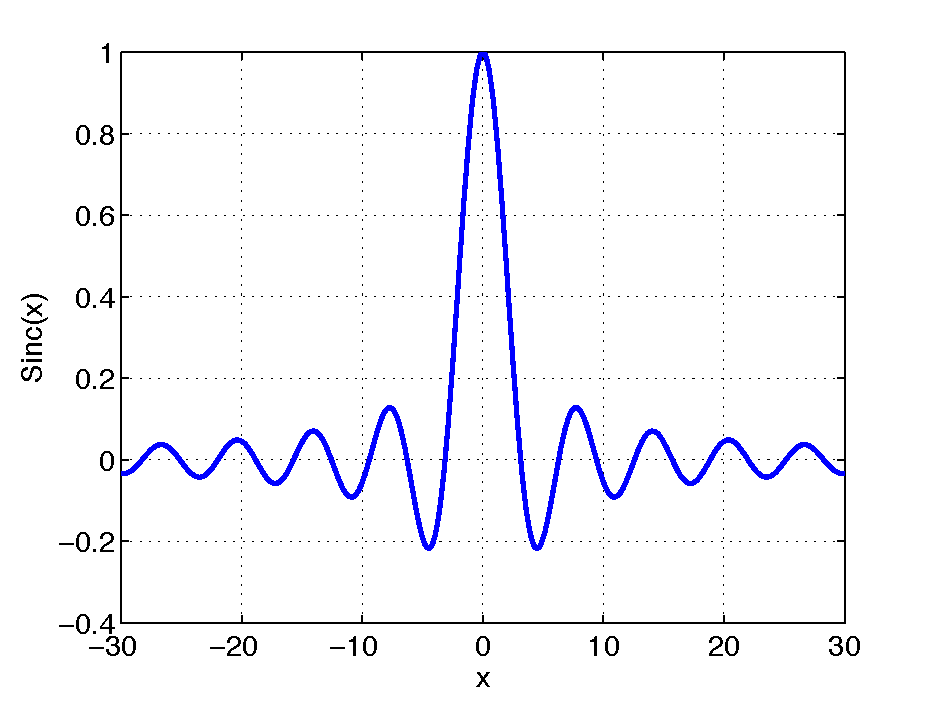
\includegraphics[width=.6\linewidth]{Figures/SincPlot}
%        \caption{Here goes the caption.}
%        \label{fig:Sinc}
%    \end{center}
%\end{figure}
%Figure~\ref{fig:Sinc} shows a shows a plot of the function $\sin(x)/x$. 
%
%If I need to make a simple diagram, I use powerpoint and select the drawing and save it as a pdf. For example, look at Figure~\ref{fig:MechaSys}.
%\begin{figure}[ht]
%    \begin{center}
%        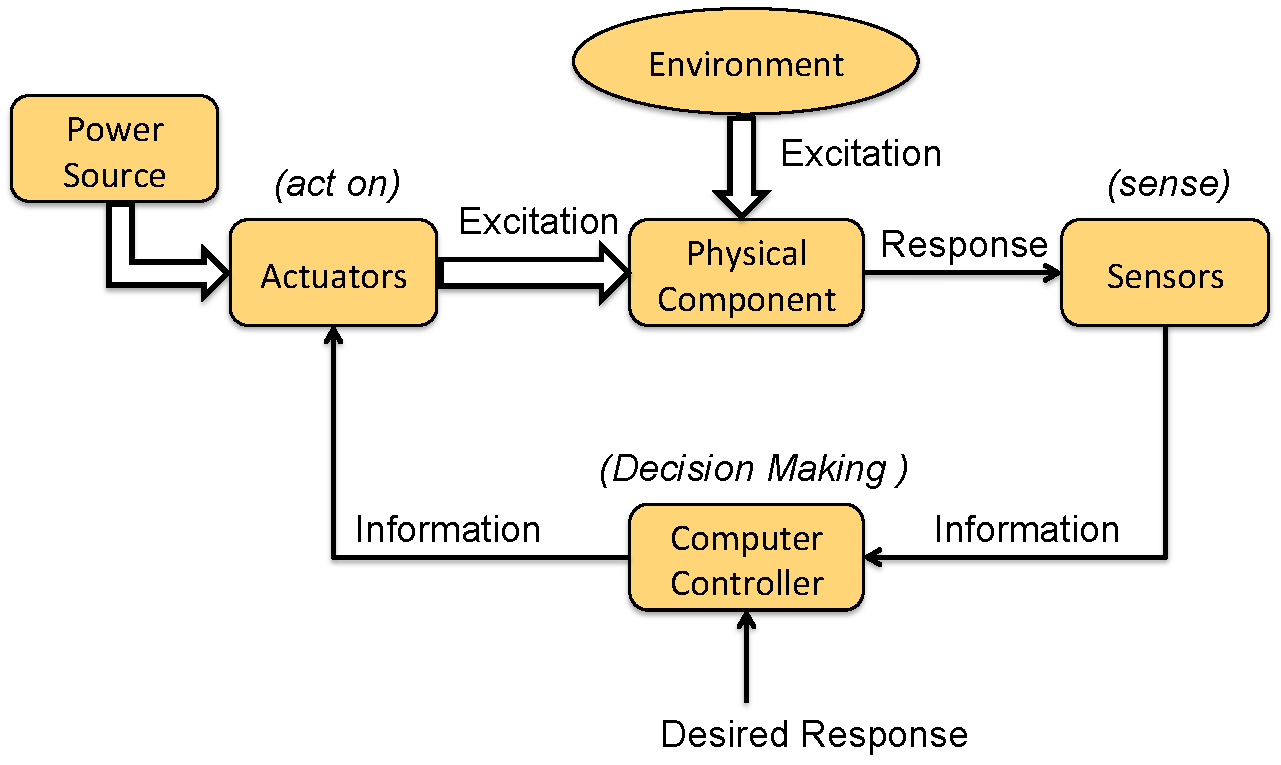
\includegraphics[width=.6\linewidth]{Figures/MechaSys}
%        \caption{Here goes the caption.}
%        \label{fig:MechaSys}
%    \end{center}
%\end{figure}
%%%%%%%%
%\newpage
%\subsection{Lists}
%To create lists use the environments \verb|itemize|, \verb|enumerate|, or \verb|description|
%
%The following is generated using \emph{itemize}
%\begin{itemize}
%    \item This is item 1 
%    \item This is item 2
%\end{itemize}
%%
%The following is generated using \emph{enumerate}
%\begin{enumerate}[1)]
%    \item This is item 1 
%    \begin{enumerate}[a)]
%        \item Subitem a
%        \item Subitem b
%        \begin{enumerate}[i)]
%            \item Subsubitem i
%            \item Subsubitem ii
%        \end{enumerate}
%    \end{enumerate}
%    \item This is item 2
%\end{enumerate}
%%
%The following is generated using \emph{description}
%\begin{description}
%    \item[foo)] This is item 1 
%    \item[bar)] This is item 2
%\end{description}
%
%\subsection{Code listings}
%
%To include a syntax-highlighted code listing, you can use the \emph{listings} package. The default options are specified by the \verb|\lstset| command. There are 3 main commands, all of which can include options to override the defaults:
%\begin{enumerate}
%    \item \verb|\lstinline|: Command for including code fragments inline with the text, as an alternative to \verb|\verb|. For example, we might describe function prototypes such as \lstinline[language=C,breaklines=true]|int main(int argc, char *argv[])|.
%    \item \verb|\begin{lstlisting}|,\ldots,\verb|\end{lstlisting}|: Environment for including a source code listing---embedded in the LaTeX source---in a box or floating environment. An example is shown in Listing~\ref{lst:sqrt}.
%    \item \verb|\lstinputlisting|: Command for including a source code listing---loaded from an external file---in a box or floating environment. This method is preferred over including the code source within the LaTeX file, since the code and its documentation can always be kept in sync. An example is shown in Listing~\ref{lst:matlabserial}.
%\end{enumerate}
%
%\begin{lstlisting}[
%    language=C,
%    float=h,
%    numbers=none,
%    xleftmargin=1cm,
%    frame=none,
%    caption={A winning entry from the 16th International Obfuscated C Code Contest, that computes the square root of its input.\label{lst:sqrt}}
%    ]
%#include <stdio.h>
%int l;int main(int o,char **O,
%int I){char c,*D=O[1];if(o>0){
%for(l=0;D[l              ];D[l
%++]-=10){D   [l++]-=120;D[l]-=
%110;while   (!main(0,O,l))D[l]
%+=   20;   putchar((D[l]+1032)
%/20   )   ;}putchar(10);}else{
%c=o+     (D[I]+82)%10-(I>l/2)*
%(D[I-l+I]+72)/10-9;D[I]+=I<0?0
%:!(o=main(c/10,O,I-1))*((c+999
%)%10-(D[I]+92)%10);}return o;}
%\end{lstlisting}
%
%\lstinputlisting[
%    language=Matlab,
%    float=h,
%    numbers=left,
%    xleftmargin=1cm,
%    frame=shadowbox,
%    caption={Matlab serial communication example.\label{lst:matlabserial}},
%    morekeywords={try,catch}
%    ]{Code/serialtest.m}
%
 %%%%%%%%%%%%%%%%%%%%%%%%%%%%%%%
\section{References and Citations}\label{sec:RefCite}
To generate the bibliography look at the end of this document in .tex file. To make reference to the bibliography use the commands \verb|\citet{}| and \verb|\citep{}| \citep{strunk2007elements}. You can combine more than one reference in a single citation \citep{troyka1999simon, jay1995write}.

True \cite{TFwebsite2}
\citet{TFwebsite2}
% \cit
% %%%%%%%%%%%%%%%%%%%%%%%%%%%%%%%%
% \bibliographystyle{ieeetr}%harvard}
% \bibliography{chris} % This is the .bib file where the bibliography database is stored
\bibliography{main} 
\bibliographystyle{harvard}

\newpage
\appendix
\section{Full Extracts of Journals}
\subsection{Journals 1}
test extract
\subsection{Journals 2}
test extract 2
\subsection{Journals 3}
test extract 3
\subsection{Journals 4}
\section{Reflection}
\section{Trade-Review of "Online vs Offline" processing}\label{sec:TradeReview}


%%%%%%%%%%%%%%%%%%%%%%%%%%%%%%%%%%%%%%%%%%%%%%%%%%%%%%%%%%%%%%%%%%%%%%%%%%%%%%%%%%%%%%%%%%%%%%%%%%%%%%%%%%%%%%%%%%%%%%%%%%%%%%%%%%%%%%%%%%%%%%%%%%%%%%%%%%%%%%%%%%%%%%%%%%%%%%%%%%%%%%%%%%%%%%%%%%%%%%%%%%%%%%%%%%%%%%%%%%%%%%%%%%%%%%%%%%%%%%%%%%%%%%%%%%%%%%%%%%%%%%%%%%%%%%%%%%%%%%%%%%%%%%%%%%%%%%%%%%%%%%%%%%%%%%%%%%%%%%%%%%%%%%%%%%%%%%%%%%%%%%%%%%%%%%%%%%%%%%%%%%%%%%%%%%%%%%%%%%%%%%%%%%%%%%%%%%%%%%%%%%%%%%%%%%%%%%%%%%%%%%%%%%%%%%%%%%%%%%%%%%%%%%%%%%%%%%%%%%%%%%%%%%%%%%%%%%%%%%%%%%%%%%%%%%%%%%%%%%%%%%%%%%%%%%%%%%%%%%%%%%%%%%%%%%%%%%%%%%%%%%%%%%%%%%%%%%%%%%%%%%%%%%%%%%%%%%%%%%%%%%%%%%%%%%%%%%%%%%%%%%%%%%%%%%%%%%%%%%%%%%%%%%%%%%%%%%%%%%%%%%%%%%%%%%%%%%%%%%%%
%%%%%%%%%%%%%%%%%%%%%%%%%%%%%%%%%%%%%%%%%%%%%%%%%%%%%%%%%%%%%%%%%%%%%%%%%%%%%%%%%%%%%%%%%%%%%%%%%%%%%%%%%%%%%%%%%%%%%%%%%%%%%%%%%%%%%%%%%%%%%%%%%%%%%%%%%%%%%%%%%%%%%%%%%%%%%%%%%%%%%%%%%%%%%%%%%%%%%%%%%%%%%%%%%%%%%%%%%%%%%%%%%%%%%%%%%%%%%%%%%%%%%%%%%%%%%%%%%%%%%%%%%%%%%%%%%%%%%%%%%%%%%%%%%%%%%%%%%%%%%%%%%%%%%%%%%%%%%%%%%%%%%%%%%%%%%%%%%%%%%%%%%%%%%%%%%%%%%%%%%%%%%%%%%%%%%%%%%%%%%%%%%%%%%%%%%%%%%%%%%%%%%%%%%%%%%%%%%%%%%%%%%%%%%%%%%%%%%%%%%%%%%%%%%%%%%%%%%%%%%%%%%%%%%%%%%%%%%%%%%%%%%%%%%%%%%%%%%%%%%%%%%%%%%%%%%%%%%%%%%%%%%%%%%%%%%%%%%%%%%%%%%%%%%%%%%%%%%%%%%%%%%%%%%%%%%%%%%%%%%%%%%%%%%%%%%%%%%%%%%%%%%%%%%%%%%%%%%%%%%%%%%%%%%%%%%%%%%%%%%%%%%%%%%%%%%%%%%%%%

\section{Writing you're not sure if you want to keep}
\subsection{Development Tools and Technologies}
Windows 10, i7-7500U and GeForce 940MX, Nvidia 1080Ti, VS Code, LaTeX, Python, Matlab, sklearn, numpy, ExtraSensory dataset, git.

Visual Studio was used for developing the Python project

\subsection{Discussion on practical aspects of IMU and Audio}

\begin{itemize}
    \item I'm not sure if it's practical to try and be recording IMU plus audio
    \item It's a case of POV; if you can record IMU, you can also record audio from the POV of your user. This theoretically suggests a higher fidelity in classification, especially in determining whether an event was local (POV) or whether it was an external event (someone else)
    \item whilst IMU is helpful, the level of understanding
\end{itemize}

Python was chosen for this project due to its ease of use, ease of analysis, ease of learning and its low maintenance. Choosing which dataset was the most difficult was not difficult for me as I have worked heavily with it and its great use cases are pretty straightforward for large data sets. In fact I even wrote a Python for it recently. Although it is still an early, immature project it works quite well for training models and will be the foundation of others as well. There are very few data in the dataset I could not predict the results from. This gives me confidence that the model is accurate from the start and can be used across all datasets and in other languages.

When the dataset was large the results tended to cluster around the 50th and 75th percentile. From this dataset I learned a bit of things. First off, the most recent observations are generally much better aligned and consistent than the average number of observations. And second this isn't a problem for every one of the training data! It seems most of the time we end up with some data which has better variance and the better alignments in the data. If these outl





To summarize what we did :
We load and processed the dataset
We got familiar with the dataset by plotting some histograms and a correlation heat map of the features
We used a deep neural network with three hidden layers each one has 256 nodes.
We used a linear activation function on the output layer
We trained the model then test it on Kaggle.
We also tested two other models
Our deep neural network was able to outscore these two models
We believe that these two models could beat the deep neural network model if we tweak their hyperparameters.https://towardsdatascience.com/deep-neural-networks-for-regression-problems-81321897ca33


\subsection{Nearest Neighbour}
Nearest Neighbour was chosen as a classification method to test against, and evaluate the other methods. Nearest Neighbour would not be used as a primary method as does not generalise well\citationneeded \footnote{https://scikit-learn.org/stable/modules/neighbors.html}



ciation:

Vaizman2017a	
Vaizman, Y., Ellis, K., and Lanckriet, G. "Recognizing Detailed Human Context In-the-Wild from Smartphones and Smartwatches". IEEE Pervasive Computing, vol. 16, no. 4, October-December 2017, pp. 62-74. doi:10.1109/MPRV.2017.3971131
*Cite this paper if you use the ExtraSensory Dataset for any publication!




sounds like dropout is great for making sure accelerometer data is used

Dropout

Unlike these methods mentioned above, dropout in my understanding is tricky but practical. Like the figure shown below, the dropout will randomly mute some neurons in the neural network and we therefore have a sparse network which hugely decreases the possibility of overfitting.More importantly, the dropout will make the weights spread over the input features instead of focusing on some features.

The possibility of muting neurons is often set as 0.5 though you can feel free to make it 0.3 or 1.0. When the dropout is 1.0, then you simply don't drop out any neurons. But our experience tells us 0.5 is usually the best choice.

After finishing the training, it is important to turn off the dropout during development and testing. Otherwise, the prediction of this model is not stable since dropout add uncertainties to it.


\newpage

\end{document}
